\documentclass[a4paper,11pt,final]{article}
\usepackage{fancyvrb, color, graphicx, hyperref, amsmath, url}
\usepackage[a4paper,width=180mm,top=20mm,bottom=20mm,bindingoffset=6mm]{geometry}

%%\usepackage{palatino}

%%\usepackage[T1]{fontenc}
%%\usepackage[utf8]{inputenc}
\usepackage{fontspec}
\usepackage{booktabs}
%%\usepackage[a4paper,text={16.5cm,25.2cm},centering]{geometry}
\usepackage{hyperref}        
\usepackage{helvet}
\hypersetup  
{   pdfauthor = {Stefano Carpita},
  pdftitle={},
  colorlinks=TRUE,
  linkcolor=black,
  citecolor=blue,
  urlcolor=blue
}

\setlength{\parindent}{0pt}
\setlength{\parskip}{1.2ex}

\title{Time series analysis: IBM stocks}
\author{Stefano Carpita \\ \url{https://github.com/sfncrp}}
\date{\today}

\begin{document}
\maketitle

\section{Objectives}

Time series: given the 50+ years long history of stock values of a company, split it into years, and study their similarities, also using clustering. Objectives: compare similarities, compute clustering. Dataset: IBM stocks (source: Yahoo Finance), includes a Python snippet to read and split the data. Dataset obtained from Yahoo!Finance service.
Sequential patterns: discover patterns over the stock value time series above. Before that, preprocess the data by splitting it into monthly time series and discretizing them in some way. Objective: find Motifs-like patterns (i.e. frequent contiguous subsequences) of length at least 4 days. Dataset: same as the point before.

\section{Introduction}

The dataset, obtained from \href{https://finance.yahoo.com/quote/IBM/history?period1=-252378000&period2=1523656800&interval=1d&filter=history&frequency=1d&guccounter=1}{Yahoo Finance} REF, includes the time history of IBM stock prices from 1962 to MESE 2018 with daily frequency.
For each day the dataset contains the opening, minimum, maximum, close and adjusted prices.
The close price is adjusted considering historical stock splits, while the adjusted values considers both splits and dividends payments.
The adjustements are done 'back in time' in order to compare the current values with the past ones.




\begin{table}[htbp]
  \centering


\begin{tabular}{lrrrrrr}
\toprule
{} &   Open &   High &    Low &  Close &    Adj &     Volume \\
Date       &        &        &        &        &        &            \\
\midrule
1962-01-02 &   7.71 &   7.71 &   7.63 &   7.63 &   0.69 &  387200.00 \\
1962-01-03 &   7.63 &   7.69 &   7.63 &   7.69 &   0.70 &  288000.00 \\
1962-01-04 &   7.69 &   7.69 &   7.61 &   7.62 &   0.69 &  256000.00 \\
1962-01-05 &   7.61 &   7.61 &   7.45 &   7.47 &   0.67 &  363200.00 \\
1962-01-08 &   7.46 &   7.46 &   7.27 &   7.33 &   0.66 &  544000.00 \\
2018-04-09 & 151.80 & 154.66 & 151.74 & 152.69 & 152.69 & 4413200.00 \\
2018-04-10 & 155.03 & 156.60 & 154.75 & 155.39 & 155.39 & 3806400.00 \\
2018-04-11 & 154.37 & 155.78 & 153.88 & 155.36 & 155.36 & 3306500.00 \\
2018-04-12 & 156.75 & 158.98 & 156.67 & 158.07 & 158.07 & 5639400.00 \\
2018-04-13 & 158.67 & 159.22 & 155.91 & 156.71 & 156.71 & 3880200.00 \\
\bottomrule
\end{tabular}


\caption{Dataset head and tail.}
\end{table}

The Open, Close and Adj stock prices time history are represented in Fig. \ref{fig:timeseries}, by using a moving average with a 30 day window.
Open and Close prices closely overlaps, while the Adj value has a similar trend but lower values. The linear correlations between all the stock prices time series have values higher than 0.99.
In Fig. \ref{fig:volumes} the smoothed Volume time history is shown. 
The prices and volumes time series are very different, with a low Pearson correlation, between 0.2-0.3.


\begin{figure}[htpb]
\center
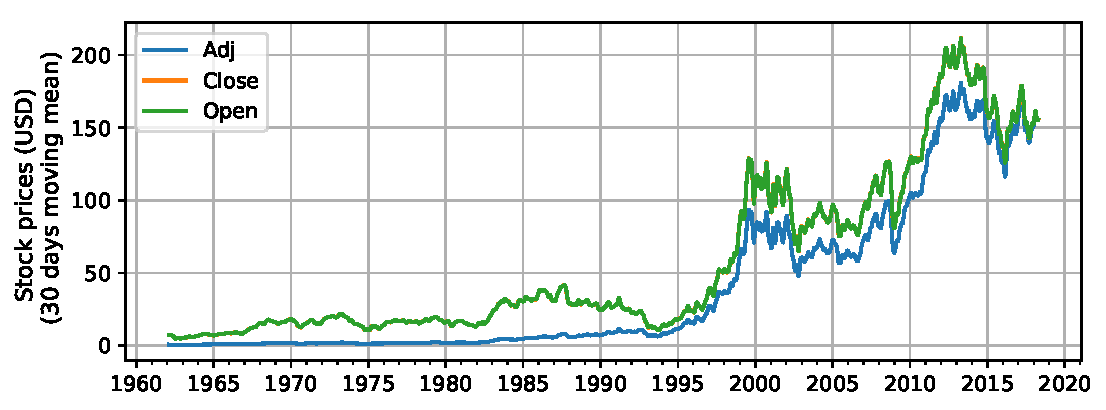
\includegraphics[width= \linewidth]{figures/report_timeseries_1.pdf}
\caption{IBM stock prices time series, values are smoothed using 30 days moving mean.}
\label{fig:timeseries}
\end{figure}



\begin{figure}[htpb]
\center
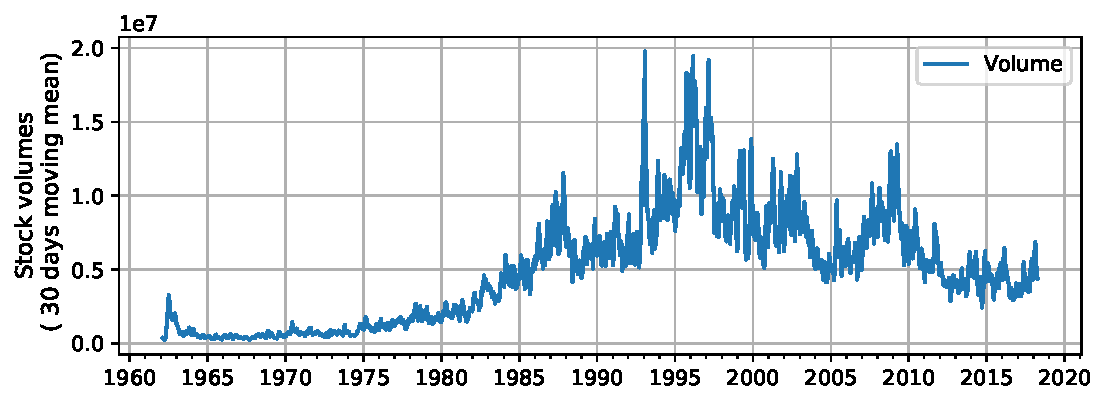
\includegraphics[width= \linewidth]{figures/report_volumes_1.pdf}
\caption{IBM volumes time history, smoothed using 30 days moving mean.}
\label{fig:volumes}
\end{figure}


\section{Year similarities}

The objective of this section is to analyze the similarities between yearly time histories of the stock prices, identifying groups of similar annual trends.
The variable used for the similarity comparison is the adjusted value Adj. The overall Adj time history has been splitted in annual time series.
The time series have been standardized obtaining annual distributions with equal zero mean and standard deviation normalized to unity. 
In order to investigate the similarity between any two annual series the Dynamic Time Warping distance has been computed. 
The DTW distance is a symmetric dissimilarity measure and not a proper mathematical distance, because generally not satisfying the triangle inequality and the positive definiteness property.
The DTW methodology permits to consider misalignment between the time series in the distance computation, which is not possible using the standard Euclidean distance. This method has an high computational cost, quadratic in the time series lengths.
In the analysis, to reduce the computational cost a Sakoe-Chiba global constraint has been used, with a band width of 80 days, corresponding about to a year quarter.
In Fig. \ref{fig:dtw_example} an example of DTW distance computation between the 2007 and 2008 time series is shown. The Adj time series are standardized and the optimal path is computed using the a Sakoe-Chiba band.



\begin{figure}[htpb]
\center
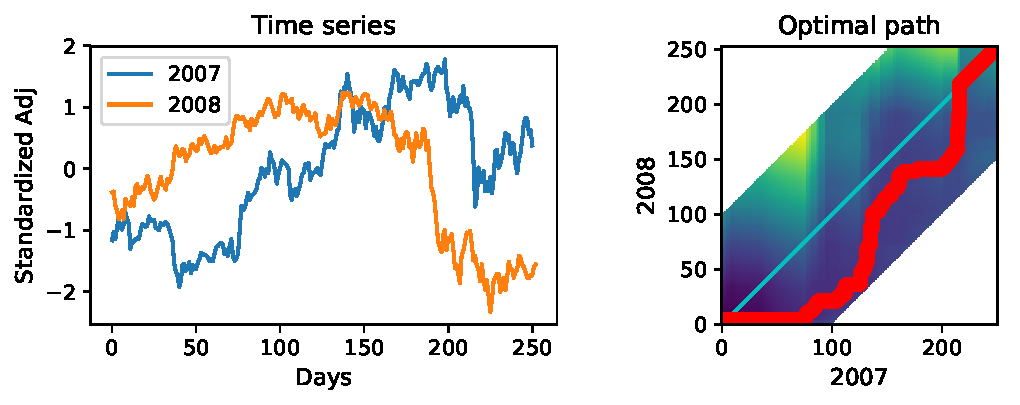
\includegraphics[width= \textwidth]{figures/report_dtw_example_1.pdf}
\caption{ 2007-2008 time series and DTW optimal path, using Sakoe-Chiba band.}
\label{fig:dtw_example}
\end{figure}








In order to identify groups of similar years, the DTW distance matrix has been computed and the DBSCAN clustering methodology applied. 
The DBSCAN algorithm has been executed multiple times, varying the radius of the neighbourhood \textit{Eps} and maintaining the minimum number of points \textit{MinPts} equal to 3. In Fig. \ref{fig:dbscan_clustering} the distances distribution is represented on the left, on the right the number of clusters as a function of the Eps value is shown. The orange curve represents the percentage of years identified as noise, normalized considering 100\% equal to the maximum number of clusters obtained. 



\begin{figure}[htpb]
\center
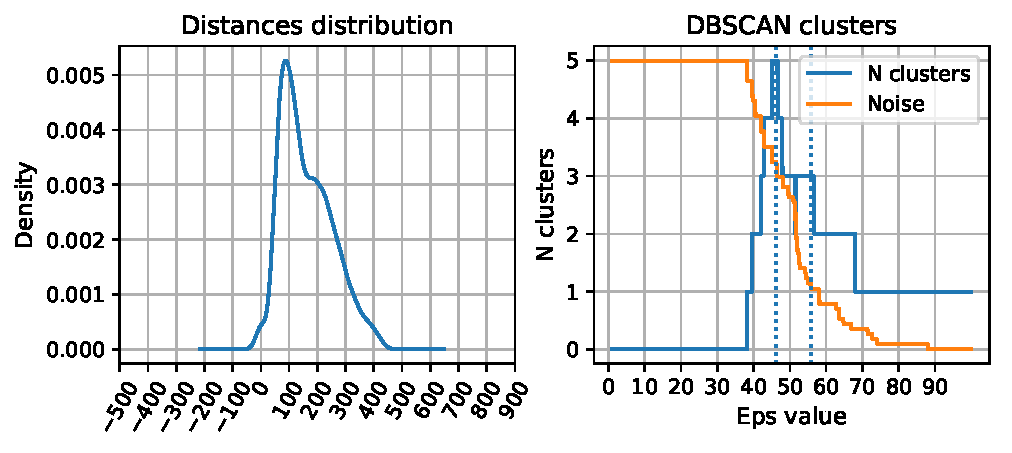
\includegraphics[width= \linewidth]{figures/report_dbscan_clustering_1.pdf}
\caption{Distances distribution and DBSCAN number of clusters vs Eps value. Percentage of noise is represented with the orange curve,   normalized considering 100\% at the maximum number of clusters obtained.}
\label{fig:dbscan_clustering}
\end{figure}



\begin{figure}[htpb]
\center
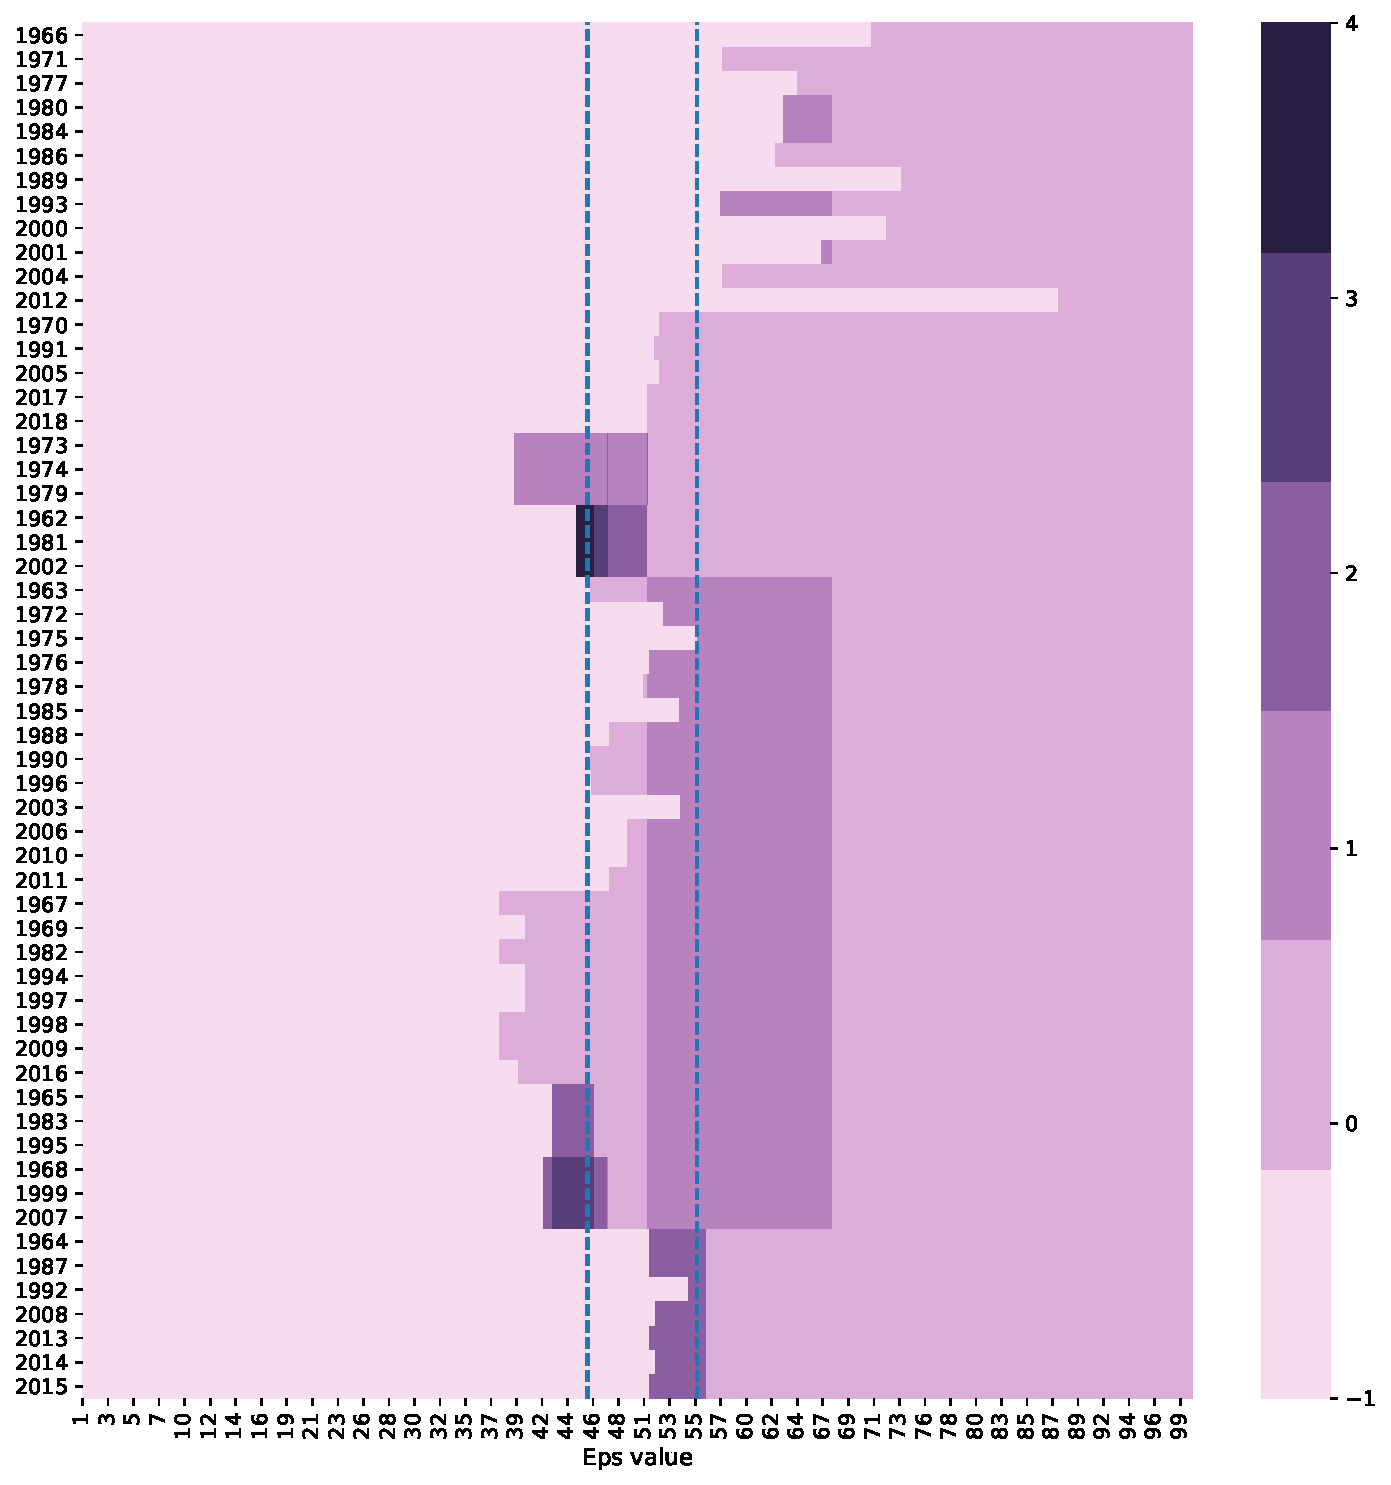
\includegraphics[width= \linewidth]{figures/report_DBSCAN_labels_1.pdf}
\caption{DBSCAN labels}
\label{fig:DBSCAN_labels}
\end{figure}


In Fig. \ref{fig:DBSCAN_labels} the colors represent the cluster labels for each year at each Eps value. The years Y-axis is ordered by considering the cluster labels at two different densities, identyfied by the vertical dotted lines. 
At Eps = 46 the years are grouped in five clusters, with more than 50\% of noise. At a lower density, corresponding to an higher Eps = 56 the time histories merged in three clusters, with about 20\% noise, as shown also in \ref{fig:dbscan_clustering}. 

The clusters 





\begin{itemize}


\item Clusters for Eps = 46: \\ 
Cluster 1:
\{ 1967, 1969, 1982, 1994, 1997, 1998, 2009, 2016\} 
 \\ Cluster 2:
\{ 1973, 1974, 1979\} 
 \\ Cluster 3:
\{ 1965, 1983, 1995\} 
 \\ Cluster 4:
\{ 1968, 1999, 2007\} 
 \\ Cluster 5:
\{ 1962, 1981, 2002\} 
 \\ \item Clusters for Eps = 56: \\ 
Cluster 1:
\{ 1970, 1991, 2005, 2017, 2018, 1973, 1974, 1979, 1962, 1981, 2002\} 
 \\ Cluster 2:
\{ 1963, 1972, 1975, 1976, 1978, 1985, 1988, 1990, 1996, 2003, 2006, 2010, 2011, 1967, 1969, 1982, 1994, 1997, 1998, 2009, 2016, 1965, 1983, 1995, 1968, 1999, 2007\} 
 \\ Cluster 3:
\{ 1964, 1987, 1992, 2008, 2013, 2014, 2015\} 
 \\ 

\end{itemize}


\begin{figure}[htpb]
\center
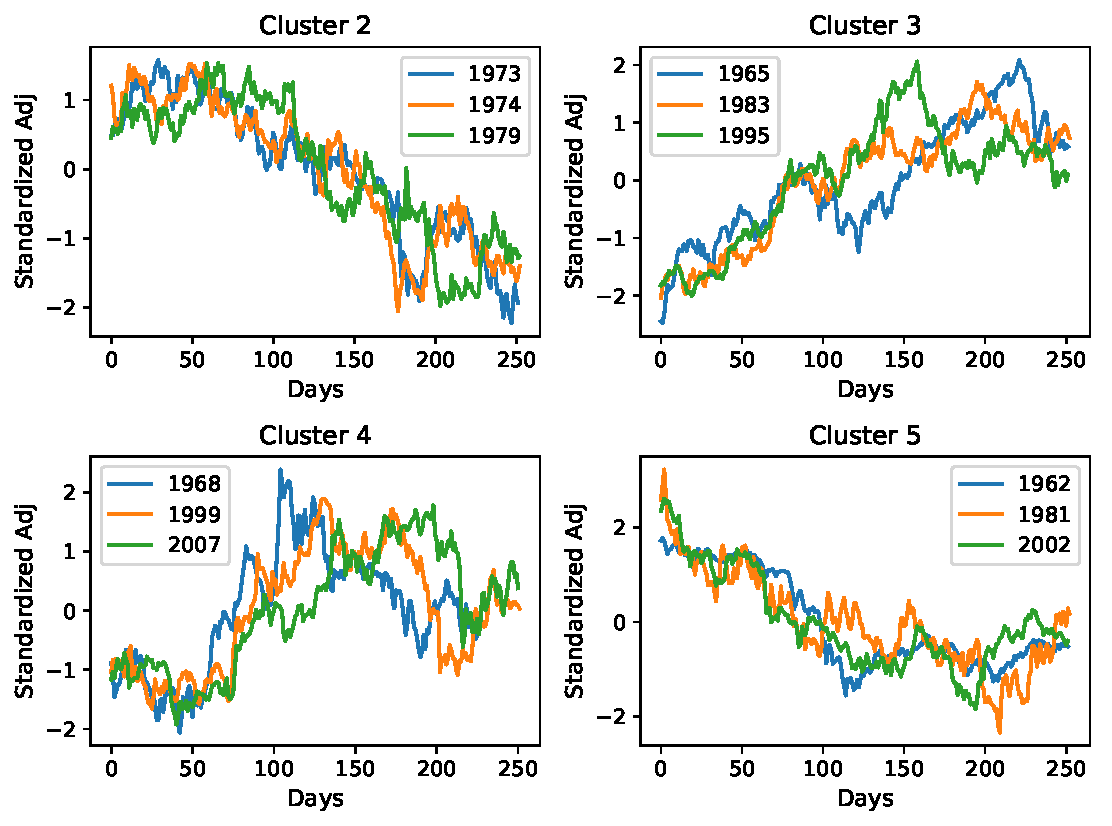
\includegraphics[width= \linewidth]{figures/report_figure12_1.pdf}
\caption{Time histories for different clusters}
\label{fig:None}
\end{figure}



Possible questions to answer:
\begin{itemize}
\item Overall description of the time series: which are the best/worse years?  
\item There is a periodicity in the best/worse years?
\item There is a periodicity during each year?
\item To which event are correlated the best/worse years? Find history 
  of the company in particular moments
  
\item What is it the average year trend over all the IBM stock history? 
\item Which year groups are most similar? Why are they similar?
\item There is a periodicity in the similarities?  
  
  
  
\end{itemize}



\end{document}
